\documentclass[tikz,border=2pt]{standalone}
% Preámbulo común de los diagramas TikZ (misma paleta y letra que las notas)
\usepackage[T1]{fontenc}\usepackage[utf8]{inputenc}
\usepackage{libertinus}\usepackage{libertinust1math}
\usepackage[defaultsans,scale=0.92]{lato}
\usepackage{amsmath,amssymb,bm}
\usepackage{tikz}\usetikzlibrary{calc,positioning,arrows.meta,shapes.geometric,decorations.pathreplacing,decorations.pathmorphing,fit,backgrounds}
\definecolor{snlazul}{HTML}{1E5AA8}\definecolor{snlnoche}{HTML}{14213D}\definecolor{snlvioleta}{HTML}{6C4AB6}
\definecolor{snlcoral}{HTML}{D1495B}\definecolor{snlambar}{HTML}{E09F3E}\definecolor{snlverde}{HTML}{2A9D8F}
\definecolor{snlteal}{HTML}{0F7173}\definecolor{snlgris}{HTML}{5C677D}\definecolor{snlfondo}{HTML}{F4F6FA}
\tikzset{>={Stealth[length=2.2mm]},
  bloque/.style={draw=#1,fill=#1!8,thick,rounded corners=2pt,minimum height=11mm,minimum width=20mm,align=center,font=\small},
  bloque/.default=snlazul,
  suma/.style={draw=snlnoche,thick,circle,inner sep=0pt,minimum size=5mm},
  flecha/.style={->,thick,draw=snlnoche},
  etq/.style={font=\small,text=snlnoche},
  nota/.style={font=\footnotesize\sffamily,text=snlgris,align=center}}

\begin{document}
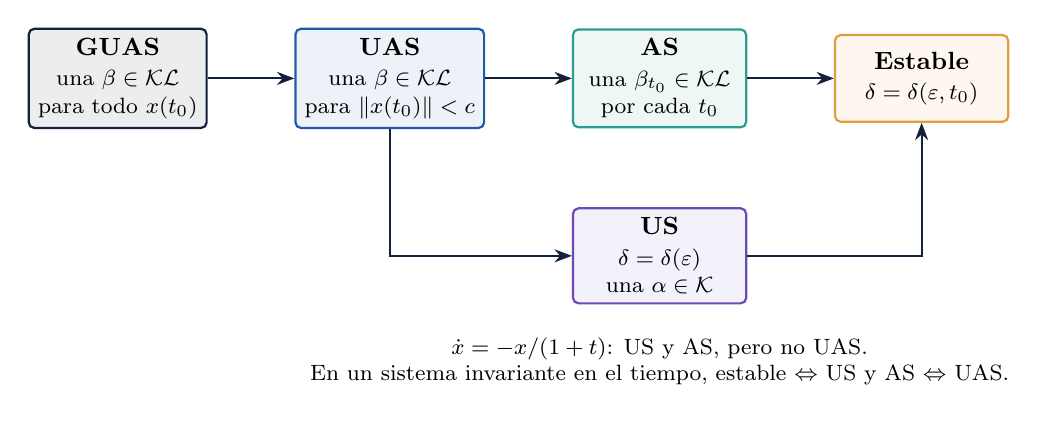
\begin{tikzpicture}[node distance=7mm and 11mm]
 \node[bloque=snlnoche,minimum width=22mm] (guas) {\textbf{GUAS}\\ \footnotesize una $\beta\in\mathcal{KL}$\\[-1pt]\footnotesize para todo $x(t_0)$};
 \node[bloque=snlazul,right=of guas,minimum width=22mm] (uas) {\textbf{UAS}\\ \footnotesize una $\beta\in\mathcal{KL}$\\[-1pt]\footnotesize para $\|x(t_0)\|<c$};
 \node[bloque=snlverde,right=of uas,minimum width=22mm] (as) {\textbf{AS}\\ \footnotesize una $\beta_{t_0}\in\mathcal{KL}$\\[-1pt]\footnotesize por cada $t_0$};
 \node[bloque=snlambar,right=of as,minimum width=22mm] (est) {\textbf{Estable}\\ \footnotesize $\delta=\delta(\varepsilon,t_0)$};
 \node[bloque=snlvioleta,below=10mm of as,minimum width=22mm] (us) {\textbf{US}\\ \footnotesize $\delta=\delta(\varepsilon)$\\[-1pt]\footnotesize una $\alpha\in\mathcal K$};
 \draw[flecha] (guas) -- (uas); \draw[flecha] (uas) -- (as); \draw[flecha] (as) -- (est);
 \draw[flecha] (uas.south) |- (us.west); \draw[flecha] (us.east) -| (est.south);
 \node[below=3mm of us,font=\footnotesize,align=center] {$\dot x=-x/(1+t)$: US y AS, pero no UAS.\\ En un sistema invariante en el tiempo, estable $\Leftrightarrow$ US y AS $\Leftrightarrow$ UAS.};
\end{tikzpicture}
\end{document}
